% Rockstar over several nodes (pegasus). Figure and table: make_rs_multinode_figure.py; data: data/rs_multinode_halos.npz.

At $2048^3$ Rockstar needs about 624\,GB (2.2 times its particle array, measured scaling from $512^3$), more than a
pegasus node (385\,GB). Rockstar has no MPI: a server process and the writer/reader clients talk over TCP sockets, and
the server records each client's address from its connection, so the single-node build runs across nodes unchanged.
\fp{job_rockstar.pbs} now does this when \texttt{RS\_NODES} $>1$: the server runs on the first node of the job and
listens on its name (instead of \texttt{localhost}), one client per node (the others started over ssh) forks
\texttt{RS\_NCPU} writers, so the particles and their memory are spread over the nodes, and the halo files go straight
to the shared \fp{HALO_DIR}. \fp{setup_production.py} sets \texttt{RS\_NODES} on pegasus to the fewest nodes that hold
$1.1\times$ the memory estimate (which already exceeds the measured peak, 1.75--1.9 times the particle array) at most
360\,GB each: 2 nodes of 344\,GB (64 writers) at $2048^3$; the runs r2 and r10 were changed to this.

\paragraph{Test.} The 101 outputs of the $128^3$, $100$\,\Mpch{} pegasus test run (the GPU end-to-end test) with the
same 64 writers in three ways on the debug queue (17 Nov 2026): 2 nodes $\times$ 32 writers (\texttt{hpc082},
\texttt{hpc083}; job 37895), one node $\times$ 64 writers (job 37896) and the latter again (job 37897). All three
finished every snapshot in 24.4--25.8\,min; the job's memory sampler on the first node saw 0.6\,GB (PSS) with 2 nodes
against 1.0\,GB on one, the share of the writers on that node. Rockstar is not deterministic from run to run (the
order in which the writers' work arrives changes the result slightly), so the 2-node catalogues are judged against
the difference between the two 1-node runs (Table~\ref{tab:rsmn}, Fig.~\ref{fig:rsmn}): matched within 50\,kpc/$h$
95--97\% of the halos in either case, 89--93\% with identical $M_{\rm vir}$, 6--9\% differing by more than 1\%, and
$N(>M_{\rm vir})$ within 0.5\% from $10^{11}$ to $10^{14}$\,\Msunh. The 2-node run differs from either 1-node run as
much as they differ from each other: running on several nodes adds no difference of its own. Above $10^{13}$\,\Msunh{}
fewer masses are bit-identical (65--80\%), but 95--100\% agree within 1\% in both comparisons.

\begin{figure}[H]
\centering
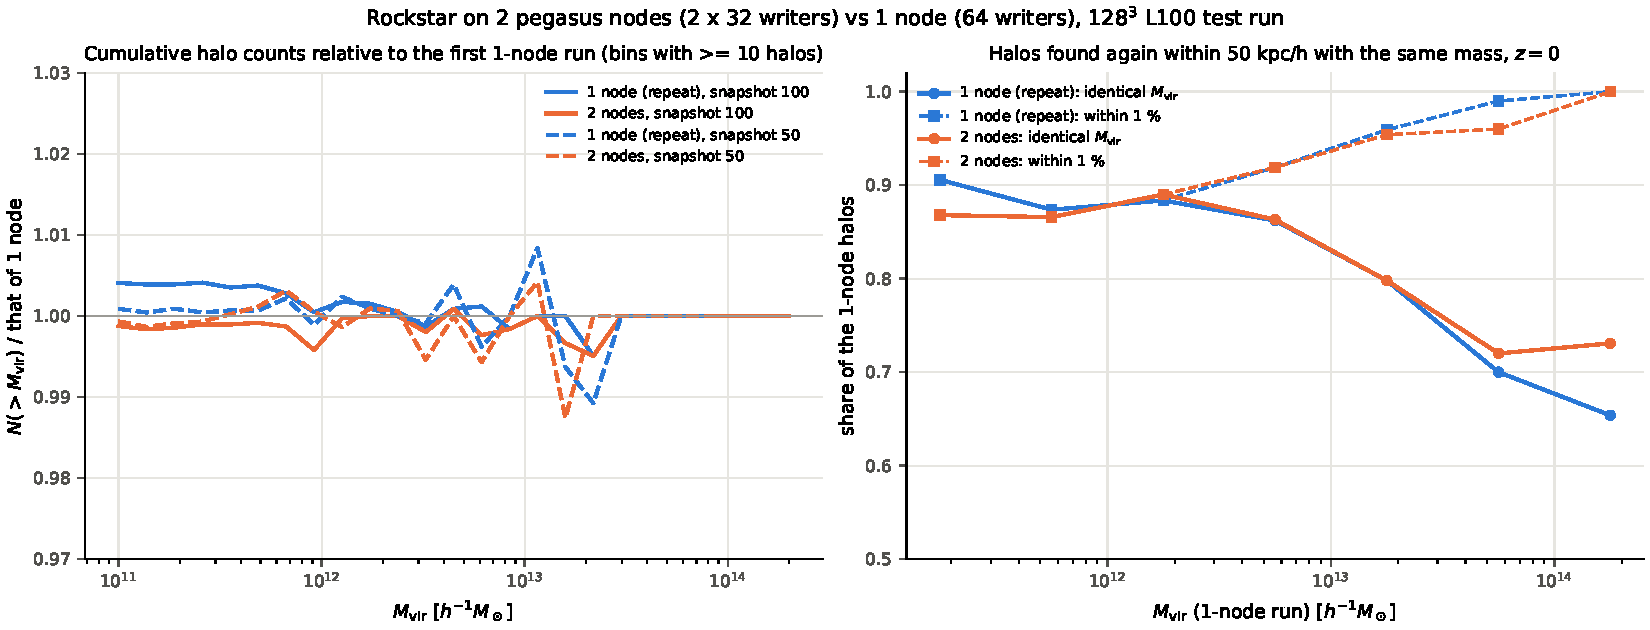
\includegraphics[width=\textwidth]{figs/rs_multinode.pdf}
\caption{Rockstar on 2 nodes (orange) and a repeated 1-node run (blue), both against the first 1-node run, all with 64
writers. Left: cumulative halo counts relative to the 1-node run at $z=0$ (solid) and snapshot 50 (dashed). Right:
share of the 1-node halos found again within 50\,kpc/$h$ with identical $M_{\rm vir}$ (solid) and within 1\% (dashed),
$z=0$.}
\label{fig:rsmn}
\end{figure}

\begin{table}[H]
\centering\footnotesize
% written by make_rs_multinode_figure.py
\begin{tabular}{cccccc}
\toprule
snapshot & runs & halos & matched [\%] & identical $M_{\rm vir}$ [\%] & $|\Delta M/M|>1\%$ [\%] \\
\midrule
30 & 1 node vs 1 node (repeat) & 2893, 2884 & 95.4 & 92.2 & 6.6 \\
30 & 1 node vs 2 nodes & 2893, 2889 & 95.1 & 91.6 & 7.2 \\
30 & 1 node (repeat) vs 2 nodes & 2884, 2889 & 94.9 & 92.5 & 6.4 \\
\midrule
50 & 1 node vs 1 node (repeat) & 4553, 4556 & 95.7 & 88.5 & 9.0 \\
50 & 1 node vs 2 nodes & 4553, 4551 & 95.5 & 88.8 & 8.8 \\
50 & 1 node (repeat) vs 2 nodes & 4556, 4551 & 95.9 & 89.5 & 7.9 \\
\midrule
80 & 1 node vs 1 node (repeat) & 5023, 5022 & 96.8 & 91.1 & 6.6 \\
80 & 1 node vs 2 nodes & 5023, 5008 & 96.3 & 90.3 & 6.5 \\
80 & 1 node (repeat) vs 2 nodes & 5022, 5008 & 96.4 & 90.2 & 6.8 \\
\midrule
100 & 1 node vs 1 node (repeat) & 4910, 4930 & 97.5 & 88.8 & 7.8 \\
100 & 1 node vs 2 nodes & 4910, 4905 & 96.9 & 89.7 & 7.1 \\
100 & 1 node (repeat) vs 2 nodes & 4930, 4905 & 96.8 & 89.2 & 7.5 \\
\bottomrule
\end{tabular}

\caption{Halo catalogues of the three Rockstar runs compared pairwise: halos matched by position within 50\,kpc/$h$,
of those the share with identical $M_{\rm vir}$ and with $|\Delta M/M| > 1\%$.}
\label{tab:rsmn}
\end{table}
